\section{DESENVOLVIMENTO}
\subsection{MATERIAIS}
Os materiais usados no trabalho foram duas bases de dados ambas da NBA Advanced Stats\footnote{National Basketball Associativo} sendo uma da \textit{season} de 2014 a 2018 com 9.840 jogos com os dados armazenados em um arquivo csv, a outra indo da \textit{season} de 2007 a 2019 com 30.000 jogos com os dados armazenados em um banco de dados e sendo acessado através da nba-api PyPI. 

A ferramenta utilizada para o desenvolvimento foi o \textit{JupyterLab}, linguagem de programação {python} e o uso das bibliotecas  pandas, numpy, \textit{sklearn}, \textit{seaborn}, matplotlib.

A NBA advances stats e um site patrocinado pela SAP com o proposito e de manter um registros de toda liga da NBA e facilitar e acesso a essa informações pelas equipes e organizações. A nba-api PyPI e uma API para acesso a www.nba.com, o principal objetivo e mapear e analisar o maior numero posivel de jogos.

O \textit{jupyterlab} é um ambiente de desenvolvimento interativo baseado na \textit{web} para \textit{notebooks}. O \textit{jupyterlab} é facil de configurar e organizar, a interface do usuário para suporta uma ampla variedade de fluxos de trabalho em ciência de dados, computação científica e aprendizado de máquina.O \textit{jupyterlab} é extensível e modular e fácil de adicionar os \textit{plug-ins}, que adicionam novos componentes e se integram aos já existentes\cite{jupyter}.

Python é uma linguagem de programação criada por Guido van Rossum em 1991. Os objetivos do projeto da linguagem eram produtividade e legibilidade, é uma linguagem de alto nível, multi paradigma, suporta o paradigma orientado a objetos, imperativo, funcional e procedural. Possui tipagem dinâmica e uma de suas principais características é permitir a fácil leitura do código e exigir poucas linhas de código se comparado ao mesmo programa em outras linguagens\cite{python}.

O pandas é uma biblioteca de código aberto, licenciada por BSD \footnote{Berkeley Software Distribution}, que fornece estruturas de dados de alto desempenho e fáceis de usar e ferramentas de análise de dados para a linguagem de programação \textit{python}. O pandas ajuda a preencher essa lacuna, permitindo que você execute todo o fluxo de trabalho de análise de dados no \textit{python} sem precisar mudar para uma linguagem\cite{pandas}.

O numPy é uma biblioteca \textit{python} que é usada para realizar cálculos em \textit{arrays} multidimensionais. Fornecendo um grande conjunto de funções e operações que ajudam os programadores a executar facilmente cálculos numéricos.\cite{numpy}

O \textit{scikit learn} é uma biblioteca \textit{python} que é usada para aprendizado de máquina. Ela possui uma variedade de algoritmos incluindo vários algoritmos de classificação, regressão e agrupamento incluindo máquinas de vetores de suporte, florestas aleatórias, \textit{gradient boosting}, \textit{k-means}\cite{scikit}.

O matplotlib é uma biblioteca de plotagem 2D do python, é uma biblioteca que tenta facilitar e facilitar a gerar gráficos, histogramas, espectros de potência, gráficos de barras, gráficos de erros, gráficos de dispersão etc\cite{matplotlib}.

O seaborn é uma biblioteca de visualização de dados Python baseada no matplotlib . Ele fornece uma interface de alto nível para desenhar gráficos estatísticos atraentes e informativos.\cite{seaborn}


\subsection{METODOLOGIA}
Os algoritmos usados para as predições são os de regressão linear, regressão logística, k-NN\footnote{k-nearest neighbors},  arvore de decisão, floresta aleatória, máquinas de vetores de suporte.

O algoritmo de regressão linear responsável por modelar uma associação entre uma ou mais variáveis de saída e entrada. O processo de regressão pode ser dividido em duas categorias, as paramétricas, no qual o relacionamento entre as variáveis é conhecido, e não paramétricas onde não existe conhecimento preexistente entre as variáveis. As técnicas de regressão linear procuram a relação entre duas variáveis por meio de uma equação de uma linha reta\cite{Bogoni2019}.

A regressão logística é uma técnica utilizada para a estimação de uma variável de natureza binária, estimando o valor em 0 ou 1, sendo que as variáveis independentes podem ser de natureza categórica ou não. Igualmente como na regressão linear é
necessário aplicar pesos onde ajustam-se aos dados de treinamento do algoritmo, porém a regressão logística não procura a melhor reta que se ajuste aos dados, mas sim a melhor curva. A regressão logística calcula uma razão de probabilidade da variável alvo, que posteriormente é convertida em uma variável de base logarítmica, permitindo assim a classificação com base na aproximação de um dos valores\cite{Witten2011}.

O algoritmo k-NN é um método não paramétrico usado para classificação e regressão . Nos dois casos, a entrada consiste nos k exemplos de treinamento a saída depende se k-NN é usado para classificação ou regressão. Na classificação k-NN, a saída é uma associação de classe. Um objeto é classificado pelo voto de pluralidade de seus vizinhos, sendo o objeto atribuído à classe mais comum entre os k vizinhos mais próximos. Os vizinhos são obtidos de um conjunto de objetos para os quais a classe ou o valor da propriedade do objeto é conhecida\cite{KamgarParsi1985}.

O processo de classificação em uma árvore de decisão, acontece de maneira recursiva, de modo que o nó inicial representa o conjunta de dados, em seguida deve ser avaliado se os objetos são da mesma classe, sendo esse o caso o nó é considerado um nó folha, caso contrário um atributo precisa ser usado para dividir os dados. Este processo deve ser executado recursivamente, ele pode ser descontinuado caso faltarem atributos para realizar testes de divisão ou caso todos os registros forem da mesma classe\cite{castro}.

Florestas aleatórias são um grupo de árvores de decisões, nos quais juntos formam uma floresta. Estas árvores são geradas com base em um atributo aleatório que é o responsável pela divisão em cada nó da árvore. A precisão de uma floresta aleatória é determinada de acordo com a força de cada classificador da árvore, e também o nível de dependência entre eles, o melhor modo de atingir essa precisão é mantendo a força dos classificadores e não aumentar a correlação entre eles\cite{castro}.

A técnica de máquinas de vetores de suporte, têm como fundamento o aprendizado em cima da estatística, o algoritmo apresenta ótima performance na utilização de dados de alta dimensionalidade. O mesmo funciona através de um conceito de hiperplano, sendo definido um limite linear neste plano para realizar a classificação, o algoritmo possuí a função de detectar o hiperplano de margem máxima, aquele com a maior margem separação entre as classes, com o objetivo de apresentar menos erros de generalização em relação a margens menores\cite{Tan2009}.

Para desenviolamento e testes foi necessário a escrita dos algoritmos,para o começo foi importadas as bibliotecas, e foi carregada as bases de dados, apos a base de dados ser carregadas em um \textit{dataframe}. foi feita a avaliação de ambas as bases e feita a escolha das características que seria usadas para a predição.

A base1\footnote{base de dados de 2014 a 2018 com 9.840} contendo 34 características sendo elas: 
\begin{table}[htbp]
	\begin{longtable}{|l|l|} \hline 
		Características              & Descrição                                                                                                                                   \\ \hline 
		team                & sigla do time                                                                                                                               \\ \hline
		game                          & id do jogo                                                                                                                                  \\ \hline
		date                         & data do jogo                                                                                                                                \\ \hline
		opponent                      & sigla do oponente                                                                                                                           \\ \hline
		winorloss                    & vitoria e derrota                                                                                                                           \\ \hline
		team points                & pontos do time                                                                                                                              \\ \hline
		opponent points               & pontos do oponente                                                                                                                          \\ \hline
		field goals                   & \begin{tabular}[c]{@{}l@{}}cesta marcada em qualquer \\ arremesso ou toque que não \\ seja lance livre\end{tabular}                         \\ \hline
		field goals attempted        & \begin{tabular}[c]{@{}l@{}}tentativa cesta marcada em \\ qualquer arremesso ou toque \\ que não seja lance livre\end{tabular}               \\ \hline
		X3 point shots               & cesta de 3 pontos                                                                                                                           \\ \hline
		X3 point shots attempted     & tentativa de cesta de 3 pontos                                                                                                              \\ \hline
		X3 point shots opp            & cesta de 3 pontos oponente                                                                                                                  \\ \hline
		X3 point shots attempted opp & \begin{tabular}[c]{@{}l@{}}tentativa de cesta de 3 pontos\\ oponente\end{tabular}                                                           \\ \hline
		free throws                 & arremessos livres                                                                                                                           \\ \hline
		free throws attempted       & tentativa de arremessos livres                                                                                                              \\ \hline
		free throws opp               & arremessos livres oponente                                                                                                                  \\ \hline
		free throws attempted opp   & \begin{tabular}[c]{@{}l@{}}tentativa de arremessos livres\\ oponente\end{tabular}                                                           \\ \hline
		rebounds                      & rebotes                                                                                                                                     \\ \hline
		Total rebounds               & total de rebotes                                                                                                                            \\ \hline
		assists                       & assistência                                                                                                                                 \\ \hline
		steals                       & roubada de bola                                                                                                                             \\ \hline
		blocks                       & bloqueio de bola                                                                                                                            \\ \hline
		turnovers                    & rotatividade                                                                                                                                \\ \hline
		total fouls                    & falta total                                                                                                                                 \\ \hline		
	\end{longtable}
\end{table}
\newpage
\begin{table}[htbp]
	\begin{longtable}{|l|l|} \hline 
		opp field goals              & \begin{tabular}[c]{@{}l@{}}cesta marcada em qualquer \\ arremesso ou toque que não \\ seja lance livre do oponente\end{tabular}             \\ \hline
		opp field goals attempted    & \begin{tabular}[c]{@{}l@{}}tentativa cesta marcada em \\ qualquer arremesso ou toque \\ que não seja lance livre do\\ oponente\end{tabular} \\ \hline
		opp off rebounds              & rebotes dos oponentes                                                                                                                       \\ \hline
		opp total rebounds           & total de rebote dos oponentes                                                                                                               \\ \hline
		opp assists                  & assistência oponente                                                                                                                        \\ \hline
		opp steals                   & roubada de bola oponente                                                                                                                    \\ \hline
		opp blocks                   & bloqueio de bola oponente                                                                                                                   \\ \hline
		opp turnovers                 & rotatividade do oponente                                                                                                                    \\ \hline
		opp total fouls              & total de faltas do oponente \\ \hline                                                                                                               
\end{longtable}
\end{table}

Depois de um analise as características que não foram relevante foram excluídas da base se dados as que foram retirada sao as \textit{team}, \textit{game}, \textit{date}, \textit{home}, \textit{opponent}.

A base2\footnote{base de dados de 2007 a 2019 com 30.000 jogos} contendo 30 características sendo elas:
\newpage

 
 Depois de um analise as características que não foram relevante foram excluídas da base se dados as que foram retirada sao as \textit{season id}, \textit{team id}, \textit{team abbreviation}, \textit{team name}, \textit{game id}, \textit{team out}, \textit{match up}, \textit{gamedate}.

Apos a retirada das características que não serão usadas foi feito um processamento nos dados, transformando as colunas \textit{(W/L)win loss} e \textit{winorloss} que continha dos dados de vitoria como "L" e derrota como "L", as linha contendo "W" foi convertida para "1" as com "L" para "0". É verificando se a dados faltantes na base de dados, caso houve-se dados faltante  as lacunas foi preenchida com a media dos dados da receptiva coluna.

Com as base de dados preparada foi feito uma divisão na base, sendo dividida em duas parte uma para teste e outra para treino, com a base de teste contendo 30 \% dos dados e a base treino contendo os outra 70 \%. com a base separa em quatro vetores sendo os vetores x\_treino, x\_teste, y\_treino, y\_teste.

Logo após a divisão dos vetores foi feita a instanciação do algoritmos que sera utilizado, foi chamada a função de treino do algoritmo. Em seguida ao treino da base ser realizado foi feita a chamada do função de predição, para mostrar os dados foi realizado um plote contendo os dados reais e o que foi previsto, também foi realizado exibição das métricas de erro do algorítimo. A seguir foi realizados a predição usando o método do \textit{Cros Validation} para ver se haveria melhoria na predição dos dados.

\subsection{RESULTADOS} 

Apos a construção dos algoritmos irei mostrar os resultados dos teste de cada algoritmo com as duas bases de dados e faz no final fazer um comparativo entre o desempenho dos algoritmos.

O algoritmo de regressão linear com a base1\footnote[4]{base de dados de 2014 a 2018 com 9.840 jogo} teve um taxa de acerto de 65\%, veja o grafico de relação entre os dados reais e os previstos. Após aplicar \textit{Cros Validation} o essa taxa teve um aumento de 2\%.
\begin{figure}[htbp]
	\begin{center}
		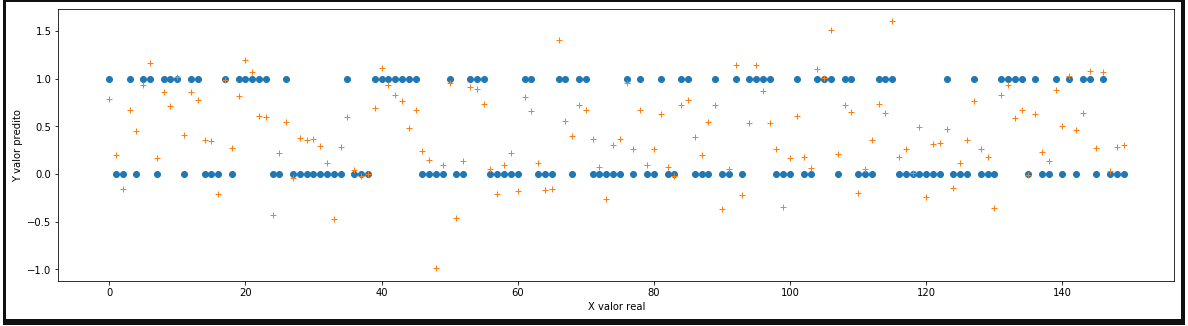
\includegraphics[width=0.7\linewidth]{imagens/regressailinear.png}\\
	\end{center}
	\caption[relação entre os dados reais e os previstos]{relação entre os dados reais e os previstos}
	\label{fig:logo}
	%%\legend{Fonte: Próprio Autor}
\end{figure}

O algoritmo de regressão linear com a base2\footnote[5]{base de dados de 2007 a 2019 com 30.000 jogos} teve um taxa de acerto de 68\%, veja o grafico de relação entre os dados reais e os previstos. Após aplicar o \textit{Cros Validation} essa taxa teve um aumento de 3.6\%.
\begin{figure}[htbp]
	\begin{center}
		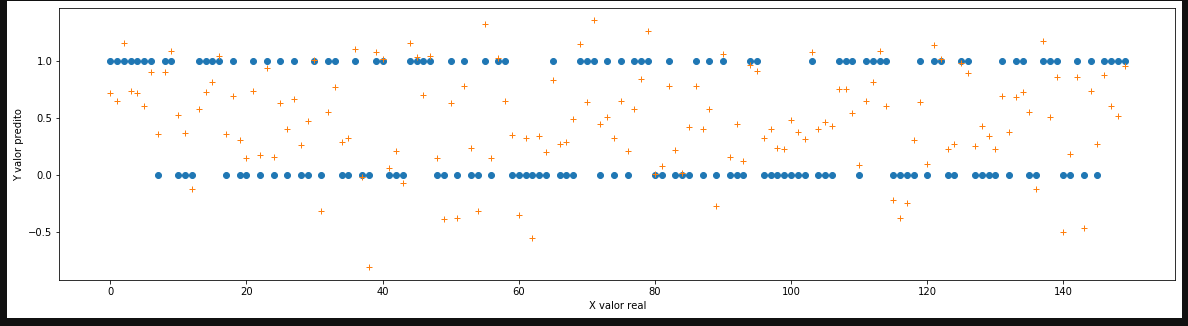
\includegraphics[width=0.7\linewidth]{imagens/regressailinearAPI.png}\\
	\end{center}
	\caption[relação entre os dados reais e os previstos]{relação entre os dados reais e os previstos}
	\label{fig:logo}
	%%\legend{Fonte: Próprio Autor}
\end{figure}

O algoritmo de arvore decisão com a base1\footnote[4]{base de dados de 2014 a 2018 com 9.840 jogo} teve um taxa de acerto de 89.7\%, veja o grafico de relação entre os dados reais e os previstos. Após aplicar o \textit{Cros Validation} essa taxa teve um aumento de 4\%.
\begin{figure}[htbp]
	\begin{center}
		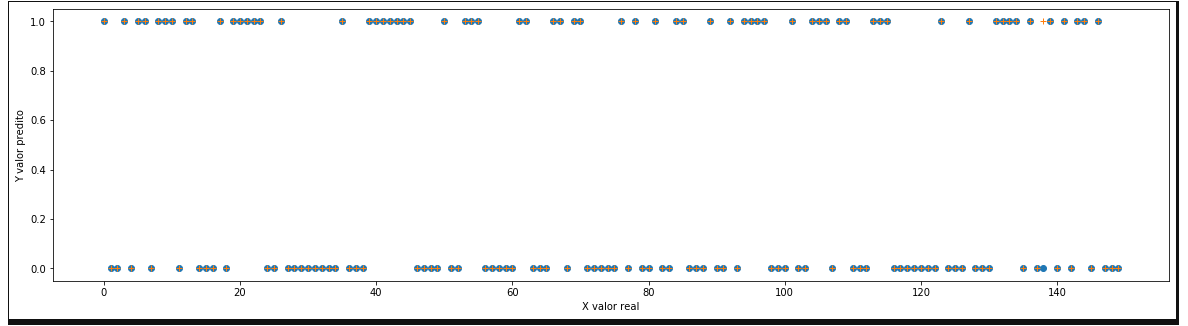
\includegraphics[width=0.7\linewidth]{imagens/arvoredecisao.png}\\
	\end{center}
	\caption[relação entre os dados reais e os previstos]{relação entre os dados reais e os previstos}
	\label{fig:logo}
	%%\legend{Fonte: Próprio Autor}
\end{figure}

O algoritmo de arvore decisão com a base2\footnote[5]{base de dados de 2007 a 2019 com 30.000 jogos} teve um taxa de acerto de 97\%, veja o grafico de relação entre os dados reais e os previstos. Após aplicar o \textit{Cros Validation} essa taxa teve um  aumento de 3\%.
\begin{figure}[htbp]
	\begin{center}
		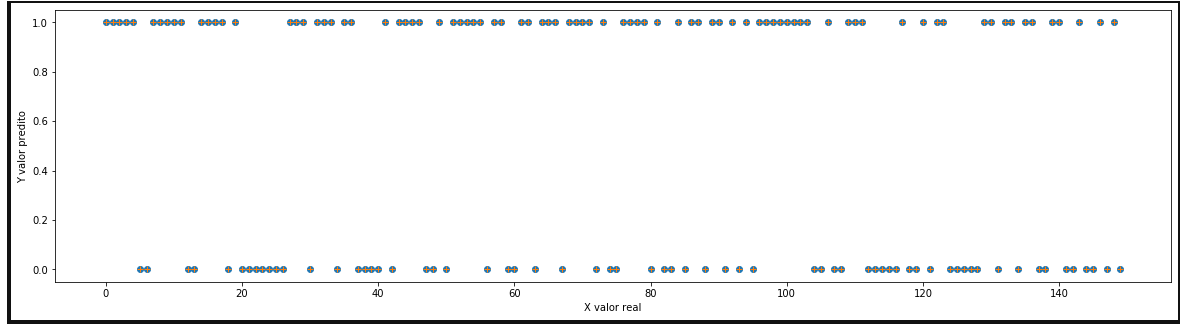
\includegraphics[width=0.7\linewidth]{imagens/arvoredecisaoAPI.png}\\
	\end{center}
	\caption[relação entre os dados reais e os previstos]{relação entre os dados reais e os previstos}
	\label{fig:logo}
	%%\legend{Fonte: Próprio Autor}
\end{figure}

O algoritmo de k-NN\footnote[3]{k-nearest neighbors} com a base1 teve um taxa de acerto de 85\%, veja o grafico de relação entre os dados reais e os previstos. Após aplicar o \textit{Cros Validation} essa taxa teve um aumento de 2.8\%.
\begin{figure}[htbp]
	\begin{center}
		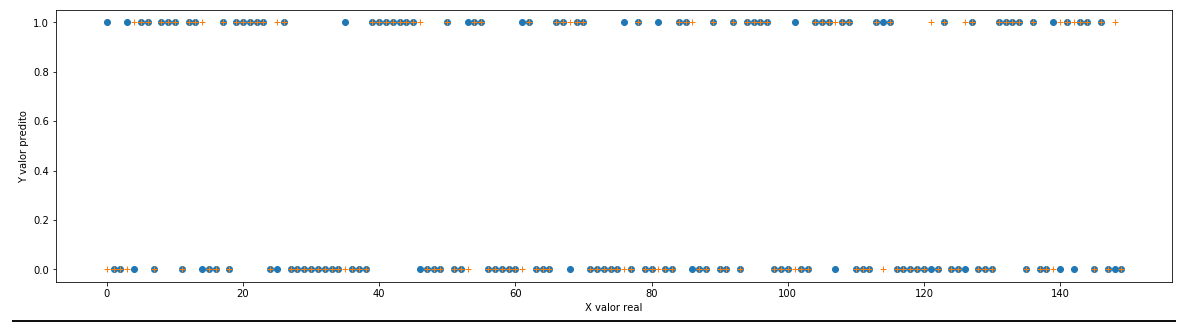
\includegraphics[width=0.7\linewidth]{imagens/knn.png}\\
	\end{center}
	\caption[relação entre os dados reais e os previstos]{relação entre os dados reais e os previstos}
	\label{fig:logo}
	%%\legend{Fonte: Próprio Autor}
\end{figure}

O algoritmo de k-NN\footnote[3]{k-nearest neighbors} com a base2\footnote[5]{base de dados de 2007 a 2019 com 30.000 jogos} teve um taxa de acerto de 87\%, veja o grafico de relação entre os dados reais e os previstos.Após aplicar o \textit{Cros Validation} essa taxa teve um aumento de 3.3\%.
\begin{figure}[htbp]
	\begin{center}
		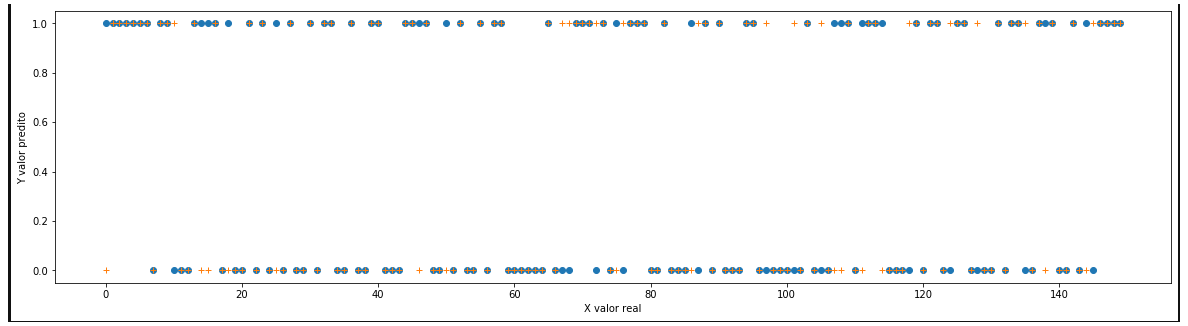
\includegraphics[width=0.7\linewidth]{imagens/knnAPI.png}\\
	\end{center}
	\caption[relação entre os dados reais e os previstos]{relação entre os dados reais e os previstos}
	\label{fig:logo}
	%%\legend{Fonte: Próprio Autor}
\end{figure}

O algoritmo de floresta aleatória com a base2 inicialmente foi testado com 10 arvores chegando a um resultado de 94\% na taxa de acerto.
\begin{figure}[htbp]
	\begin{center}
		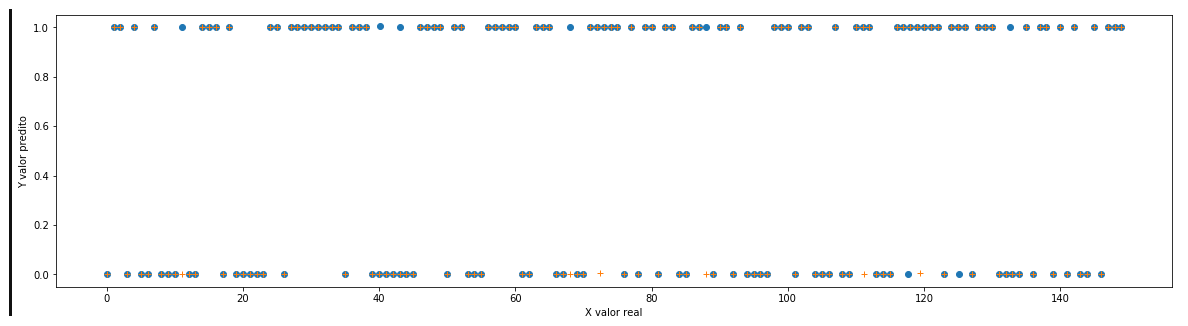
\includegraphics[width=0.7\linewidth]{imagens/florestaaleatoria.png}\\
	\end{center}
	\caption[relação entre os dados reais e os previstos com 10 arvores]{relação entre os dados reais e os previstos com 10 arvores}
	\label{fig:logo}
	%%\legend{Fonte: Próprio Autor}
\end{figure}

O algoritmo de floresta aleatória com a base2 o teste com 53 arvores o teste conseguiu atingir uma faixa de os 99\% e 100\% de precisão. Para sempre ter um taxa contante de 100\% de acerto são necessária mais de 100 arvores.
\begin{figure}[htbp]
	\begin{center}
		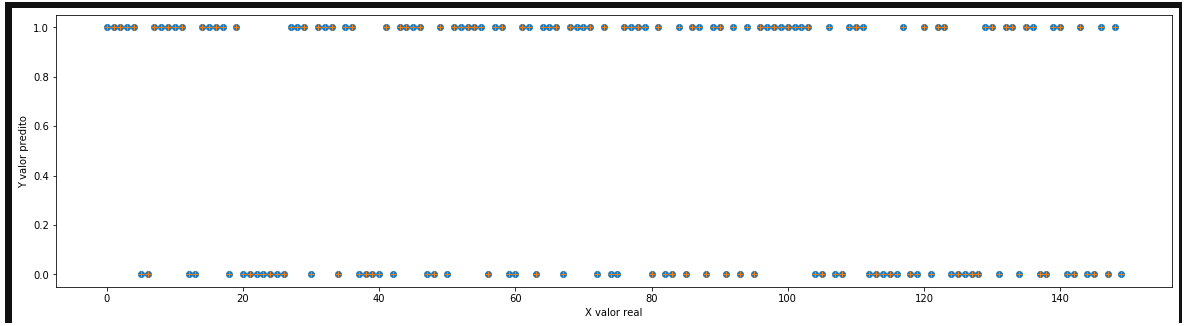
\includegraphics[width=0.7\linewidth]{imagens/florestaaleatoriaAPI.png}\\
	\end{center}
	\caption[relação entre os dados reais e os previstos com 53 arvores]{relação entre os dados reais e os previstos com 53 arvores}
	\label{fig:logo}
	%%\legend{Fonte: Próprio Autor}
\end{figure}
\newpage
O algoritmo de regressão logística tanto com a base1\footnote[4]{base de dados de 2014 a 2018 com 9.840 jogo} é com a  base2\footnote[5]{base de dados de 2007 a 2019 com 30.000 jogos} teve um taxa de acerto de 100\%, veja o grafico de relação entre os dados reais e os previstos.
\begin{figure}[htbp]
	\begin{center}
		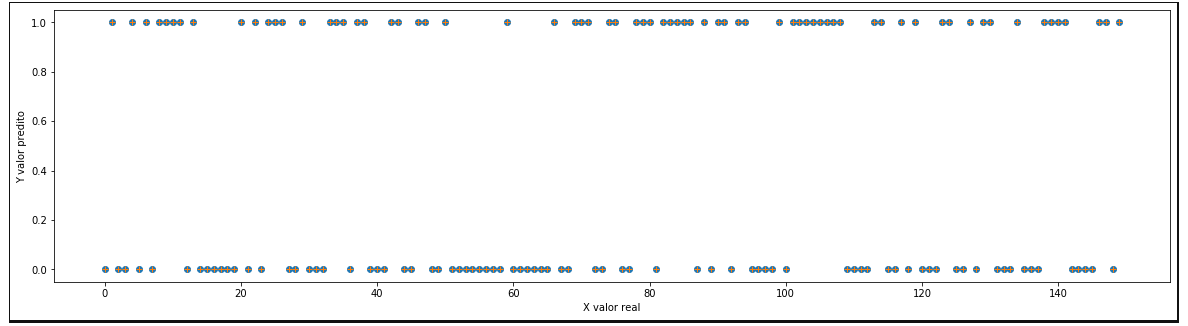
\includegraphics[width=0.7\linewidth]{imagens/regressaologistocaAPI.png}\\
	\end{center}
	\caption[relação entre os dados reais e os previstos]{relação entre os dados reais e os previstos}
	\label{fig:logo}
	%%\legend{Fonte: Próprio Autor}
\end{figure}

O algoritmo de máquinas de vetores de suporte com a base1 teve um taxa de acerto de 80\%, veja o grafico de relação entre os dados reais e os previstos.
\begin{figure}[htbp]
	\begin{center}
		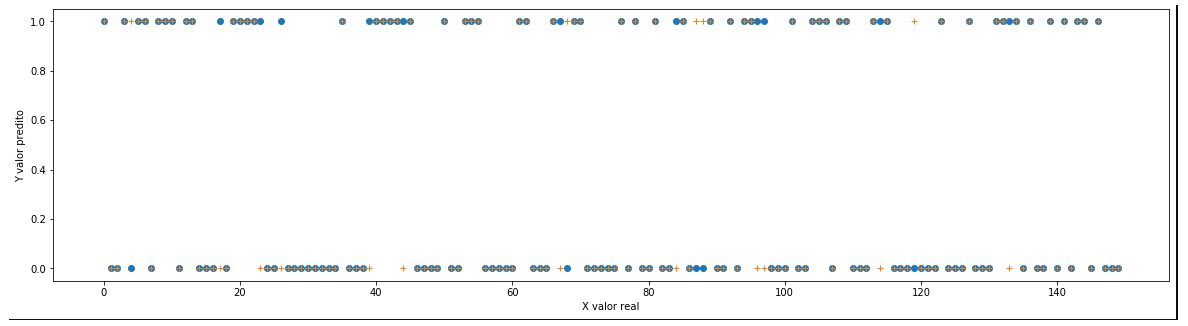
\includegraphics[width=0.7\linewidth]{imagens/SVM.png}\\
	\end{center}
	\caption[relação entre os dados reais e os previstos]{relação entre os dados reais e os previstos}
	\label{fig:logo}
	%%\legend{Fonte: Próprio Autor}
\end{figure}

O algoritmo de máquinas de vetores de suporte com a base1 teve um taxa de acerto de 87\%, veja o grafico de relação entre os dados reais e os previstos.
\begin{figure}[htbp]
	\begin{center}
		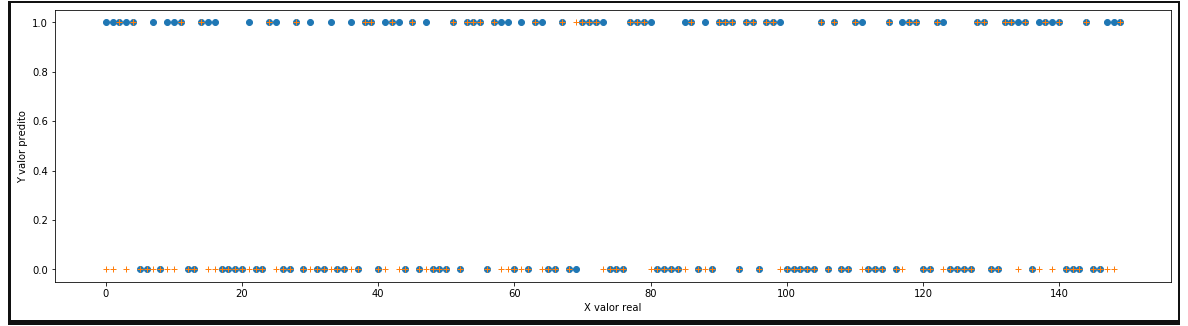
\includegraphics[width=0.7\linewidth]{imagens/SVMAPI.png}\\
	\end{center}
	\caption[relação entre os dados reais e os previstos]{relação entre os dados reais e os previstos}
	\label{fig:logo}
	%%\legend{Fonte: Próprio Autor}
\end{figure}


